\documentclass[10pt]{article}
\usepackage{amsmath, amssymb}
\usepackage{graphicx}

\begin{document}

\begin{center}
    \LARGE {Problem Set 3 – Loss Functions and Fitting Models} \\[1em]
    \Large{DS542 – DL4DS} \\[0.5em]
    \large Spring, 2025 \\
    \large Sicheng Yi (Tiger Yi)
\end{center}

\vspace{2em}

\noindent\textbf{Note:} Refer to the equations in the \textit{Understanding Deep Learning} textbook to solve the following problems.

\vspace{2em}

\section*{Problem 5.9}
Consider a multivariate regression problem in which we predict the height of an individual in meters and their weight in kilos from some data $x$. Here, the units take quite different values. What problems do you see this causing? Propose two solutions to these problems.

\noindent Answer:

\noindent Problems: Difference in variance between Height (1.5 - 2.0 m) and Weight (50 - 100 kg). The variation in weight is a lot larger than height, this will lead to class unbalance in training.  Also the weight will have a lot more influence in the loss function than height. 

\noindent Solutions: standardize the data as in $y=\frac{x-\mu}{\sigma}$  where $\mu$ is the mean and $\sigma$ is the standard deviation. Also for the loss function we can scale the weight different than the height: $L = \lambda_1 (h - \hat{h})^2 + \lambda_1 (w - \hat{w})^2 $ 



\vspace{5em}


\newpage

\section*{Problem 6.6}
Which of the functions in Figure~6.11 from the book is convex? Justify your answer. Characterize each of the points 1--7 as (i) a local minimum, (ii) the global minimum, or (iii) neither.


\begin{figure}[h]
    \centering
    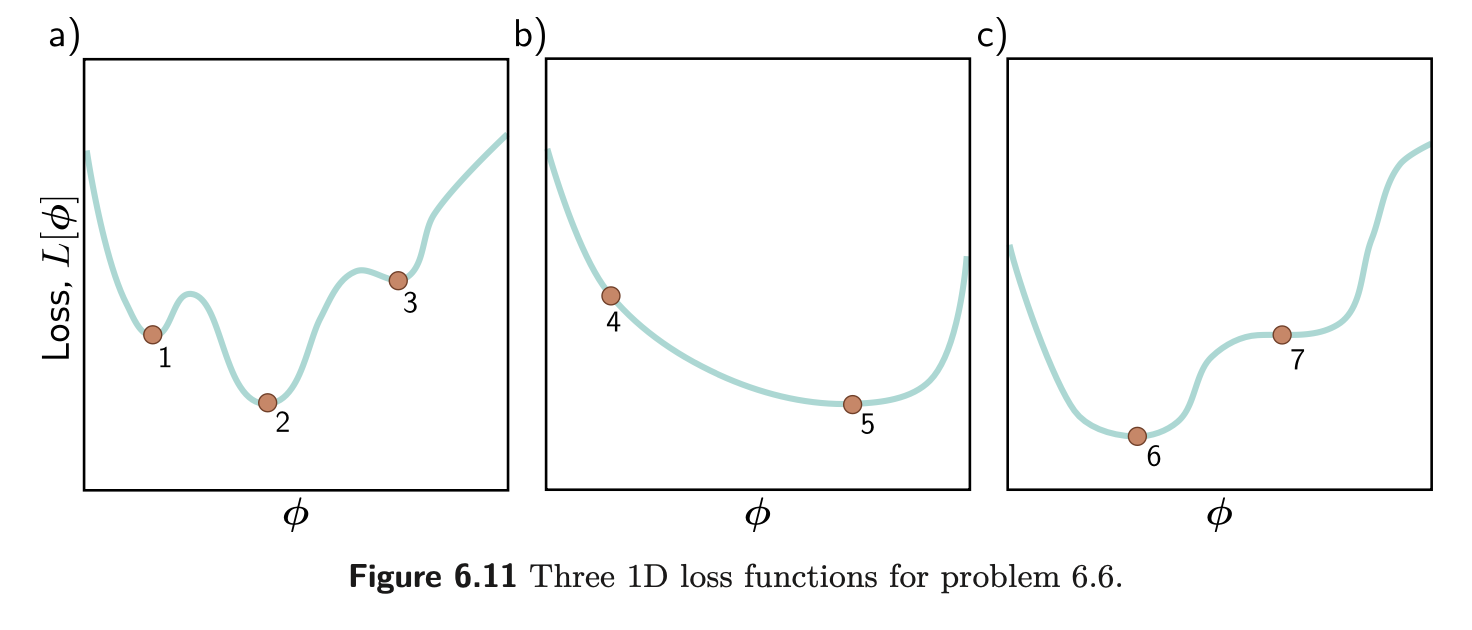
\includegraphics[width=1\textwidth]{figure.png}
    \caption{problem 6.6}
    \label{fig:problem66}
\end{figure}


\noindent Answer: 


\noindent Part 1: Only 2nd graph (b) is convex. (a) and  (c) are not convex. A convex function satisfies the property that a line segment connecting any two points on the function lies above or on the curve, and only (b) satisfy. 

\noindent Part 2: 

\noindent point 1 is local minimum 

\noindent point 2 is global minimum 

\noindent point 3 is local minimum 

\noindent point 4 is neither

\noindent point 5 is global minimum 

\noindent point 6 is global minimum 

\noindent point 7 is neither (saddle point) 




\vspace{5em}

\newpage

\section*{Problem 6.10}

Show that the momentum term \( m_t \) (equation (6.11)) is an infinite weighted sum of the gradients at the previous iterations and derive an expression for the coefficients (weights) of that sum.


\begin{figure}[h]
    \centering
    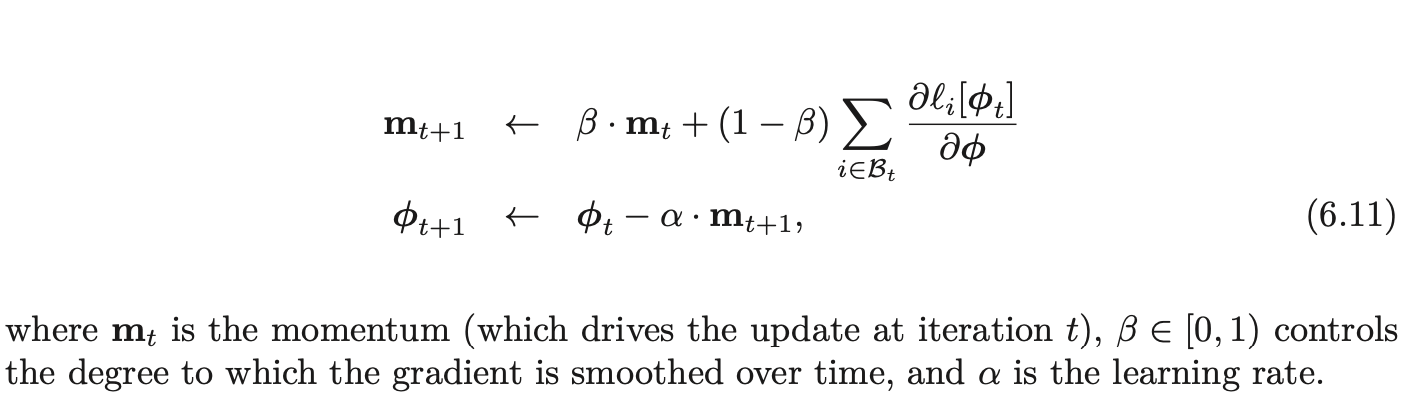
\includegraphics[width=1\textwidth]{equation.png}
    \caption{problem 6.10}
    \label{fig:problem610}
\end{figure}


\noindent Answer: 


\[
\mathbf{m}_{t+1} = \beta \mathbf{m}_t + (1 - \beta) \sum_{i \in \mathcal{B}_t} \frac{\partial \ell_i [\boldsymbol{\phi}_t]}{\partial \boldsymbol{\phi}}
\]

\noindent Expanding \( \mathbf{m}_t \) recursively:

\[
\mathbf{m}_t = \beta \mathbf{m}_{t-1} + (1 - \beta) \sum_{i \in \mathcal{B}_{t-1}} \frac{\partial \ell_i [\boldsymbol{\phi}_{t-1}]}{\partial \boldsymbol{\phi}}
\]

\noindent Substituting \( \mathbf{m}_{t-1} \):

\[
\mathbf{m}_t = \beta \left( \beta \mathbf{m}_{t-2} + (1 - \beta) \sum_{i \in \mathcal{B}_{t-2}} \frac{\partial \ell_i [\boldsymbol{\phi}_{t-2}]}{\partial \boldsymbol{\phi}} \right) + (1 - \beta) \sum_{i \in \mathcal{B}_{t-1}} \frac{\partial \ell_i [\boldsymbol{\phi}_{t-1}]}{\partial \boldsymbol{\phi}}
\]

\[
= \beta^2 \mathbf{m}_{t-2} + (1 - \beta) \sum_{i \in \mathcal{B}_{t-2}} \beta \frac{\partial \ell_i [\boldsymbol{\phi}_{t-2}]}{\partial \boldsymbol{\phi}} + (1 - \beta) \sum_{i \in \mathcal{B}_{t-1}} \frac{\partial \ell_i [\boldsymbol{\phi}_{t-1}]}{\partial \boldsymbol{\phi}}
\]

\noindent Continuing this expansion back to \( \mathbf{m}_0 = 0 \) (assuming zero initialization):

\[
\mathbf{m}_t = (1 - \beta) \sum_{k=0}^{t} \beta^{t-k} \sum_{i \in \mathcal{B}_k} \frac{\partial \ell_i [\boldsymbol{\phi}_k]}{\partial \boldsymbol{\phi}}
\]

\noindent This equation shows that \( \mathbf{m}_t \) is a weighted sum of all past gradients, where the weight assigned to the gradient at iteration k is  \( w_k = (1 - \beta) \beta^{t-k} \). 

\ 

\noindent These weights form a decaying geometric series, meaning that more recent gradients are given larger weights, and older gradients contribute less.

\ 

\noindent Conclusion: Expression for the Coefficients

\noindent The weight assigned to the gradient at iteration \( k \) is:

\[
w_k = (1 - \beta) \beta^{t-k}
\]

\noindent These weights sum to 1 in the infinite limit, ensuring that the momentum term remains a properly scaled moving average of past gradients.







\end{document}
